\section{Methods (20 points, 350 words)}
\label{sec:methods}
% Describe the methods used. How it works. It can include algorithms, system descriptions, new language constructs, analyses, etc.
% Provide diagrams to help in the discussion. Figure \ref{fig:one-col-figure} and Figure \ref{fig:two-col-figure} shows an example of a one-column figure and a two-column figure. 
% \begin{figure}
%     \centering
%     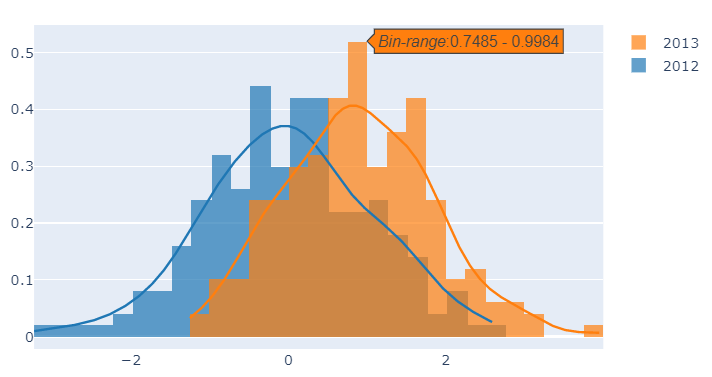
\includegraphics[width=\linewidth]{figures/example_plot.png}
%     \caption{One-column figure that explains the steps or framework of your method / model.}
%     \label{fig:one-col-figure}
% \end{figure}

% \begin{figure*}
%     \centering
%     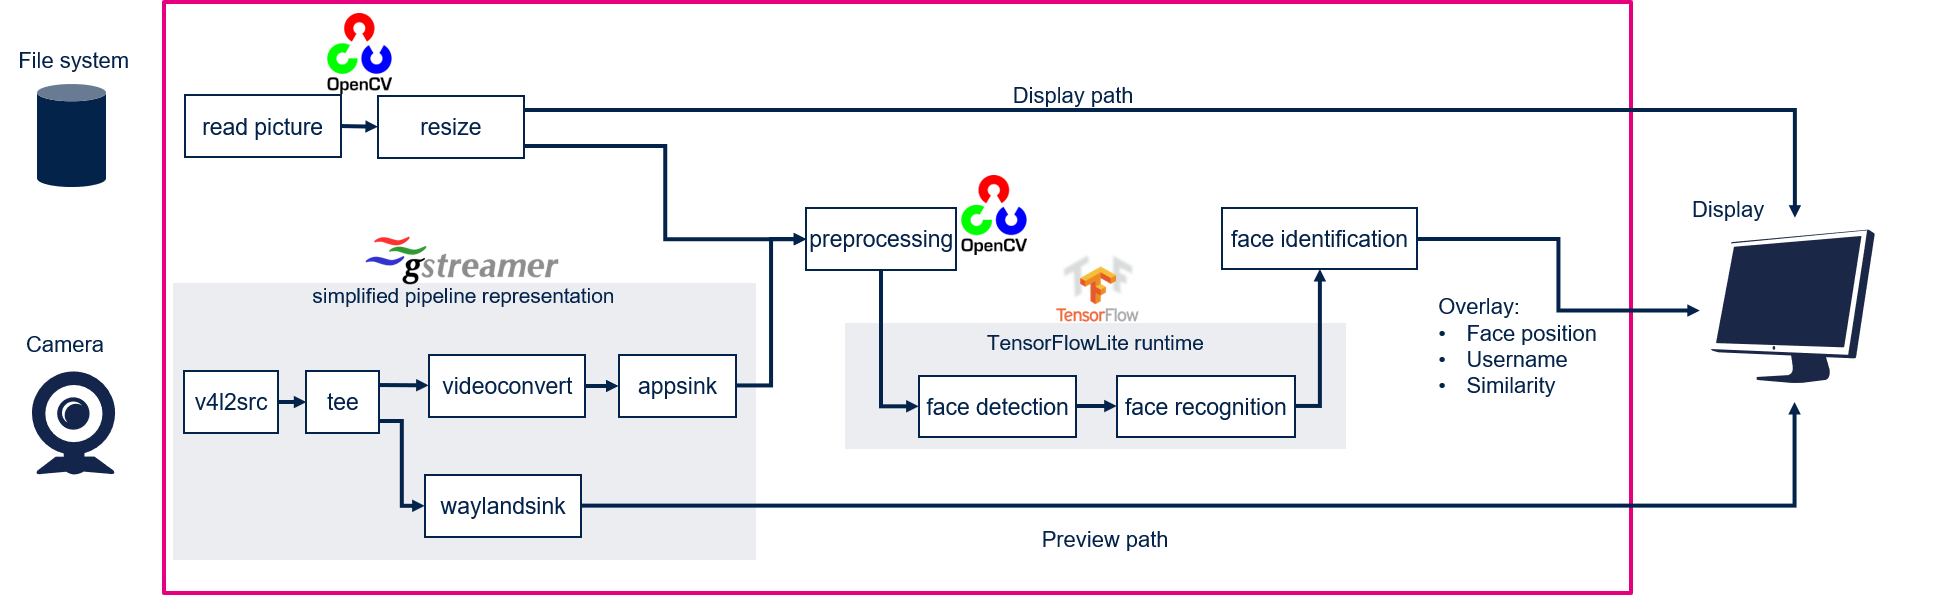
\includegraphics[width=\linewidth]{figures/example_pipeline.png}
%     \caption{One-column figure that explains the steps or framework of your method / model.}
%     \label{fig:two-col-figure}
% \end{figure*}


% \textbf{Points:} \textit{Everything concerning the methods used to solve this problem}
% \begin{itemize}
%     \item Is the method well formalized/explained?
%     \item Is the method complex/innovative?
%     \item Is the method explaining the objective function?
%     \item Are more variations of the methods considered?
% \end{itemize}



% = PARAGRAPH 1 - Overview of the evaluation pipeline

% Briefly explain that the method reuses the existing automatic_eval.py pipeline from the COMET-ATOMIC-2020 repository, and that no model retraining was performed. Clarify the input: the pregenerated BART output file (BART-atomic_2020.json) containing greedy-decoded tails for the ATOMIC2020 test set, paired against reference tails from test.tsv. This satisfies the rubric's requirement to explain what the method is actually doing

Long fuckass paragraph dummy bitch fuck ass.


% = PARAGRAPH 2 - Partitioning strategy

Explain how each test example was assigned a category based on its relation type, using the three-way taxonomy from \citet{hwang2021cometatomic}: social-interaction, physical-entity, and event-centred (you can find them in Table 1 in the original paper). Mention that scores were accumulated both at the individual relation level (23 types) and aggregated up to the category level. This is where you explain the core methodological choice \textemdash{} partitioning \textemdash{} an why the three-category split was chosen over alternatives like query length or output length. (It's because I believe the 3 different category types represent 3 entirely different types of general knowledge and have to also be evaluated as a group rather than only all 23 seperate)

% = PARAGRAPH 3 - Object function / scoring

Explain BLEU-1 through BLEU-4 as the evaluation metrics, and why all four variants are reported rather than just one (apparently in the original paper they only show BLEU-1) %TODO) VERIFY THIS
Importantly, mention that \verb|none| responses are excluded from scoring, following the convention already present in the original code. This addresses the rubric's requirement to explain the objective function.

% = PARAGRAPH 4 - Variations considered

Briefly mention the two levels of granularity as variations of the same methods: per-relation (fine-grained, 23 groups) versus per-category (coarse-grained, 3 groups). You could also note that query-length or output-length partitioning were considered as alternative strategies but that relation type was chosen because it maps directly onto the knowledge graph structure and is most directly comparable to the paper's own per-relation human evaluation in Table 3.